%To compile as handout, use
%pdflatex "\def\ishandout{1} \input{filename.tex}"
%Defaults to non-handout mode (with slide reveals)
\ifdefined\ishandout
  \documentclass[handout]{beamer}
\else
  \documentclass{beamer}
\fi
 
\usepackage{econ103slides} 

\date{Lecture \# 1}
\begin{document} 


%%%%%%%%%%%%%%%%%%%%%%%%%%%%%%%%%%%%%%%%

\begin{frame}[plain]
	\titlepage 
	

\end{frame} 


%%%%%%%%%%%%%%%%%%%%%%%%%%%%%%%%%%%%%%%%%
%\begin{frame}
	%
	%\begin{center}
		%\Huge Econ 103 -- Know Your Meme
	%\end{center}
%\end{frame}
%%%%%%%%%%%%%%%%%%%%%%%%%%%%%%%%%%%%%%%%%
%\begin{frame}
%
%\begin{figure}
%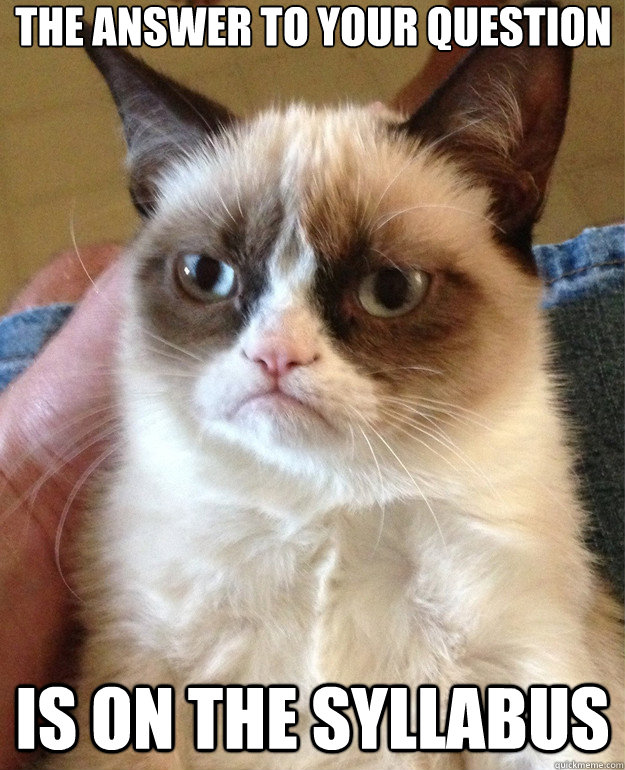
\includegraphics[scale=0.33]{./images/SyllabusMeme.jpg}
%\end{figure}
%
%
%\end{frame}
%%%%%%%%%%%%%%%%%%%%%%%%%%%%%%%%%%%%%%%%%
%\begin{frame}
%
%\begin{figure}
%
\includegraphics[scale=0.5]{./images/ResponseCardMeme.jpg}
%\end{figure}
%
%
%\end{frame}
%%%%%%%%%%%%%%%%%%%%%%%%%%%%%%%%%%%%%%%%%
%\begin{frame}
%
%\begin{figure}
%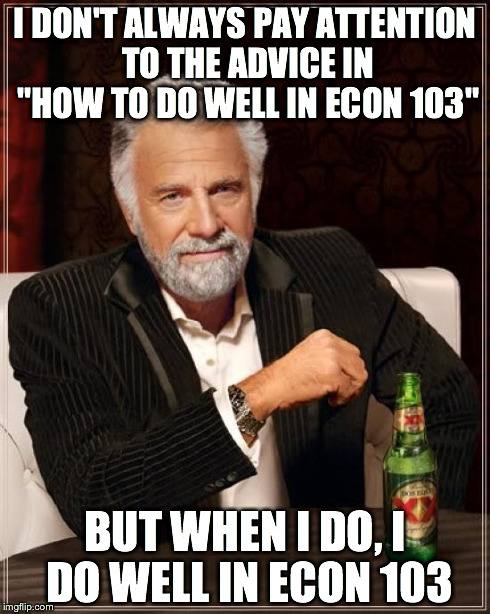
\includegraphics[scale=0.4]{./images/DoWellMeme.jpg}
%\end{figure}
%
%
%\end{frame}
%%%%%%%%%%%%%%%%%%%%%%%%%%%%%%%%%%%%%%%%%
%\begin{frame}
%
%\begin{figure}
%
\includegraphics[scale=0.5]{./images/HomeworkMeme.jpg}
%\end{figure}
%
%
%\end{frame}
%%%%%%%%%%%%%%%%%%%%%%%%%%%%%%%%%%%%%%%%%
%\begin{frame}
%
%\begin{figure}
%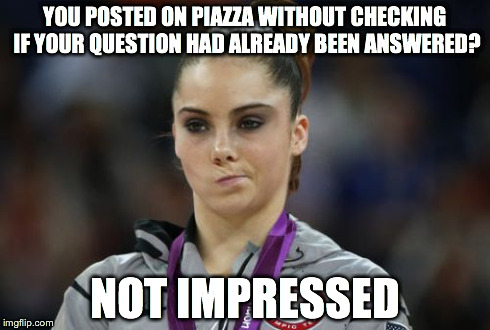
\includegraphics[scale=0.5]{./images/PiazzaMeme.jpg}
%\end{figure}
%
%
%\end{frame}
%%%%%%%%%%%%%%%%%%%%%%%%%%%%%%%%%%%%%%%%%
%\begin{frame}
%
%\begin{figure}
%
\includegraphics[scale=0.4]{./images/LaptopMeme.jpg}
%\end{figure}
%
%
%\end{frame}
%%%%%%%%%%%%%%%%%%%%%%%%%%%%%%%%%%%%%%%%%
%\begin{frame}
%\frametitle{What You Need to Know \emph{Right Now}}
%
%\begin{enumerate}
	%\item Lecture Recordings on Canvas
	%\item Log onto Piazza via Canvas 
	%\item Course Email: \texttt{econ103@ditraglia.com}
	%\item R Tutorial \#1 and Problem Set \#1
	%\item Recitations begin \emph{THIS WEEK} (Math Diagnostic)
%\end{enumerate}
%
%\end{frame}
%%%%%%%%%%%%%%%%%%%%%%%%%%%%%%%%%%%%%%%%

\begin{frame}

\frametitle{
\includegraphics[scale = 0.05]{./images/clicker} \hfill  Racial Bias in Criminal Sentencing}

Do you think there is racial bias in criminal sentencing? That is, do you think that judges may assign different sentences purely based on the race of the defendant?

\begin{enumerate}[(a)]
	\item Yes
	\item No
\end{enumerate}
%Please respond using your remote.

\end{frame}

%%%%%%%%%%%%%%%%%%%%%%%%%%%%%%%%%%%%%%%%


\begin{frame}
\frametitle{This Course: Use Sample to Learn About Population}


\begin{block}{Population}
Complete set of all items that interest investigator
\end{block}


\begin{block}{Sample}
Observed subset, or portion, of a population
\end{block}

\begin{block}{Sample Size}
\# of items in the sample, typically denoted $n$
\end{block}


\begin{block}{\hfill Examples...}\end{block}

\end{frame}


%%%%%%%%%%%%%%%%%%%%%%%%%%%%%%%%%%%%%%%%

\begin{frame}

\frametitle{In Particular: Use Statistic to Learn about Parameter}

\begin{block}{Parameter}
Numerical measure that describes specific characteristic of a population.
\end{block}

\begin{block}{Statistic}
Numerical measure that describes specific characteristic of sample.
\end{block}

\begin{block}{\hfill Examples...}\end{block}

\end{frame}

%%%%%%%%%%%%%%%%%%%%%%%%%%%%%%%%%%%%%%%%

\begin{frame}
\frametitle{Essential Distinction You Must Remember!}
\begin{figure}
\centering
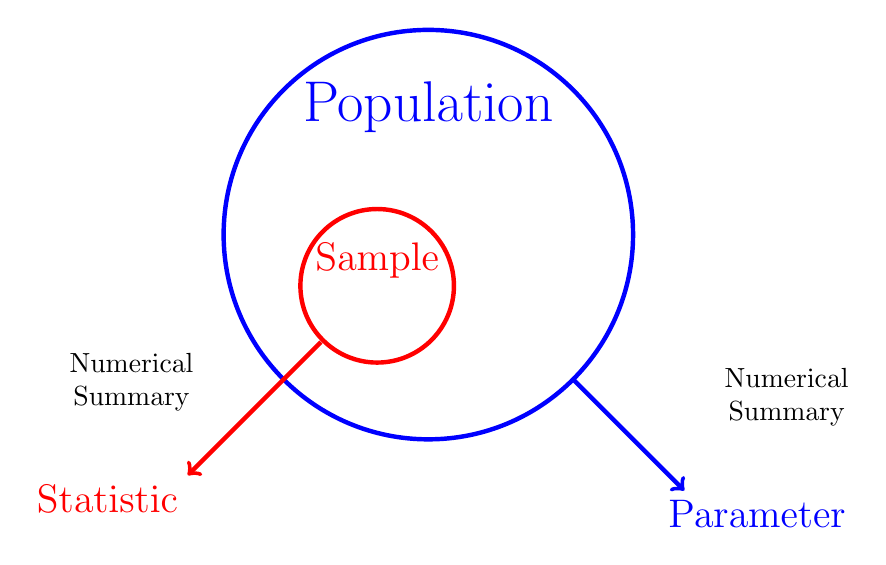
\begin{tikzpicture}[scale=1.3]
	\draw [blue, ultra thick] (0,0) circle [radius=2];
	\node [blue, font=\huge] at (0,1.25) {Population};
	\draw [blue, ultra thick, ->] (1.4,-1.4) -- (2.5,-2.5);
	\draw [red, ultra thick] (-0.5, -0.5) circle [radius=0.75];
	\node at (3.5,-1.4) {Numerical};
	\node at (3.5,-1.75) {Summary};
	\node [blue, font =\Large, below right] at (2.25, -2.5) {Parameter};
	\node [red, font=\Large] at (-0.5, -0.25) {Sample};
	\draw [red, ultra thick, ->] (-1.05, -1.05) -- (-2.35, -2.35);
	\node at (-2.9,-1.25) {Numerical};
	\node at (-2.9,-1.6) {Summary}; 
	\node [red, font =\Large, below left] at (-2.35, -2.35) {Statistic};
	
\end{tikzpicture}
\end{figure}
\end{frame}

%%%%%%%%%%%%%%%%%%%%%%%%%%%%%%%%%%%%%%%%


\begin{frame}

\frametitle{The Field of Statistics}

\begin{block}{Descriptive Statistics}
Graphical and numerical procedures to summarize data.
\end{block}


\begin{block}{Inferential Statistics}
Using data to estimate, predict, quantify uncertainty.
\end{block}


\end{frame}
%%%%%%%%%%%%%%%%%%%%%%%%%%%%%%%%%%%%%%%%

\begin{frame}

\frametitle{This Course}

\begin{enumerate}
	\item Descriptive Statistics: summarize data
		\begin{itemize}
			\item Summary Statistics
			\item Graphics
		\end{itemize}
	\item Probability: Population $\rightarrow$ Sample
		\begin{itemize}
			\item deductive: ``safe'' argument
				\begin{itemize}
					\item All ravens are black. Mordecai is a raven, so Mordecai is black.
				\end{itemize}
		\end{itemize}
	\item Statistics: Sample $\rightarrow$ Population
		\begin{itemize}
			\item inductive: ``risky'' argument
				\begin{itemize}
					\item I've only every seen black ravens, so all ravens must be black.
				\end{itemize}
		 \end{itemize}
\end{enumerate}


\end{frame}
%%%%%%%%%%%%%%%%%%%%%%%%%%%%%%%%%%%%%%%%
\begin{frame}
\frametitle{Sampling and Nonsampling Error}
In statistics we use samples to learn about populations, but samples almost never be \emph{exactly} like the population they are drawn from.
	\begin{enumerate}
		\item Sampling Error 
			\begin{itemize}
				\item \emph{Random} differences between sample and population
				\item Cancel out on average
				\item Decreases as sample size grows
			\end{itemize}
		\item Nonsampling Error
			\begin{itemize}
				\item \emph{Systematic} differences between sample and population 
				\item Does \emph{not} cancel out on average
				\item Does \emph{not} decrease as sample size grows
			\end{itemize}
	\end{enumerate}
\end{frame}



%%%%%%%%%%%%%%%%%%%%%%%%%%%%%%%%%%%%%%%%
\begin{frame}
\begin{center}
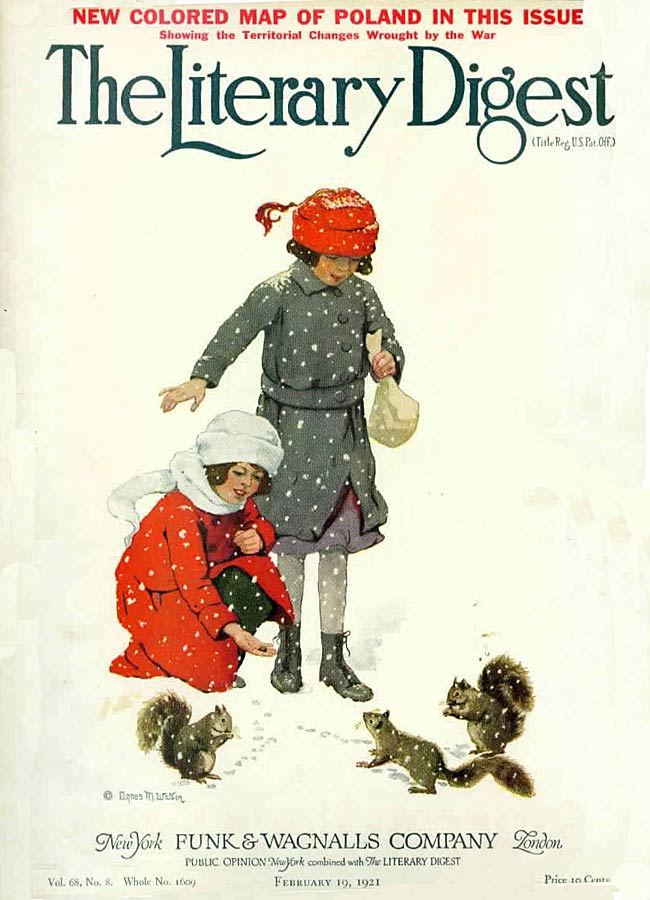
\includegraphics[scale = 0.28]{./images/LiteraryDigest}
\end{center}

\end{frame}

%%%%%%%%%%%%%%%%%%%%%%%%%%%%%%%%%%%%%%%%
\begin{frame}

\frametitle{Literary Digest -- 1936 Presidential Election Poll}

\begin{center}
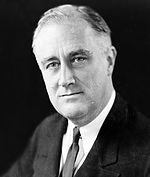
\includegraphics[scale = 0.3]{./images/FDR}
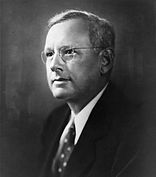
\includegraphics[scale = 1.67]{./images/Landon}\\
\small FDR versus Kansas Gov.\ Alf Landon
\end{center}

\normalsize

\begin{block}{Huge Sample}
Sent out over 10 million ballots; 2.4 million replies! (Compared to  less than $45$ million votes cast in actual election)
\end{block}

\begin{block}{Prediction}
Landslide for Landon: \emph{Landonslide},  if you will.
\end{block}
\end{frame}

%%%%%%%%%%%%%%%%%%%%%%%%%%%%%%%%%%%%%%%%
\begin{frame}
\frametitle{Spectacularly Mistaken!}

\begin{center}
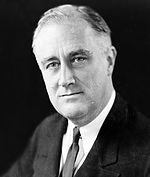
\includegraphics[scale = 0.3]{./images/FDR}
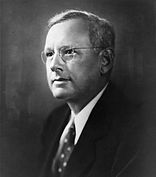
\includegraphics[scale = 1.67]{./images/Landon}\\
\small FDR versus Kansas Gov.\ Alf Landon
\end{center}

\normalsize

\begin{table}
\begin{tabular}{lcc}
&Roosevelt&Landon\\
Literary Digest Prediction: &41\% & \alert{57\%}\\
Actual Result: &\alert{61\%} & 37\%

\end{tabular}

\end{table}

\end{frame}
%%%%%%%%%%%%%%%%%%%%%%%%%%%%%%%%%%%%%%%%
\begin{frame}

\frametitle{What Went Wrong? \emph{Non-sampling Error (aka Bias)}}
\framesubtitle{Source: \href{http://www.jstor.org/stable/10.2307/2749114}{\fbox{Squire (1988)}}}

\begin{block}{Biased Sample}
Some units more likely to be sampled than others.
	\begin{itemize}
		\item Ballots mailed those on auto reg.\ list and in phone books.
	\end{itemize}
\end{block}

\begin{block}{Non-response Bias}
Even if sample is unbiased, can't force people to reply.
	\begin{itemize}
		\item Among those who recieved a ballot, Landon supporters were more likely to reply.
	\end{itemize}
\end{block}
\alert{In this case, neither effect \emph{alone} was enough to throw off the result but together they did.}
\end{frame}
%%%%%%%%%%%%%%%%%%%%%%%%%%%%%%%%%%%%%%%%
\begin{frame}
\frametitle{Randomize to Get an Unbiased Sample}

\begin{block}{Simple Random Sample}

Each member of population is chosen strictly by chance, so that: (1) selection of one individual doesn't influence selection of any other, (2) each individual is just as likely to be chosen, (3) every possible sample of size $n$ has the same chance of selection.

\end{block}

\begin{block}{What about non-response bias?}
\end{block}
\end{frame}
%%%%%%%%%%%%%%%%%%%%%%%%%%%%%%%%%%%%%%%%

\begin{frame}
\frametitle{``Americans Divided on Outlook for Next Generation''}
\framesubtitle{Source: \href{http://www.gallup.com/poll/159737/americans-divided-outlook-next-generation.aspx}{\fbox{Gallup}}}
\vspace{1em}
\begin{quote}
PRINCETON, NJ -- Americans are evenly divided about whether it is likely (49\%) or unlikely (50\%) that the next generation of youth in the country will have a better life than their parents. That is a slightly more positive assessment than in early 2011, when the slight majority, 55\%, thought it was unlikely the next generation would achieve this goal.
\end{quote}
\end{frame}

%%%%%%%%%%%%%%%%%%%%%%%%%%%%%%%%%%%%%%%%
\begin{frame}
\frametitle{Example of Sampling Error}
``...evenly divided about whether it is likely (49\%) or unlikely (50\%) that the next generation of youth in the country will have a better life...''

\vspace{2em}
\begin{quote}
Results for this USA Today/Gallup poll are based on telephone interviews conducted Dec. 14-17, 2012, with a \alert{random sample of 1025 adults}, aged 18 and older, living in all 50 U.S. states and the District of Columbia. For results based on the total sample of national adults, one can say with \alert{95\% confidence that the maximum margin of sampling error is ±4 percentage points}.
\end{quote}
\end{frame}
%%%%%%%%%%%%%%%%%%%%%%%%%%%%%%%%%%%%%%%%
\begin{frame}
\frametitle{Quantifying Sampling Error}
\framesubtitle{95\% Confidence Interval for Poll Based on Random Sample}
	$$Margin of Error (ME) \approx 2 \sqrt{P(1-P)/n}$$
	We Report: $P \pm ME$
\end{frame}

%%%%%%%%%%%%%%%%%%%%%%%%%%%%%%%%%%%%%%%%
\begin{frame}
\frametitle{
\includegraphics[scale = 0.05]{./images/clicker} \hfill Survey to find effect of Polio Vaccine}
Ask random sample of parents if they vaccinated their kids or not and if the kids later developed polio. Compare those who were vaccinated to those who weren't.

\vspace{1em}


Would this procedure:
	\begin{enumerate}[(a)]
		\item Overstate effectiveness of vaccine
		\item Correctly identify effectiveness of vaccine
		\item Understate effectiveness of vaccine
	\end{enumerate}
	%Please respond with your remote. 

\end{frame}

%%%%%%%%%%%%%%%%%%%%%%%%%%%%%%%%%%%%%%%%
\begin{frame}
\frametitle{Problem}
	Parents who vaccinate their kids may differ systematically from those who don't in \emph{other ways} that impact child's chance of contracting polio!
	
	\vspace{2em}
	\begin{alertblock}{Wealth is related to vaccination \emph{and} whether child grows up in a hygenic environment.}
	\end{alertblock}
\end{frame}
%%%%%%%%%%%%%%%%%%%%%%%%%%%%%%%%%%%%%%%%
\begin{frame}
\frametitle{Confounder}

Factor than influences both outcomes and whether subjects are treated or not. Masks true effect of treatment.
\end{frame}
%%%%%%%%%%%%%%%%%%%%%%%%%%%%%%%%%%%%%%%%


\begin{frame}

\frametitle{Experiment Using Random Assignment: Randomized Experiment}
Treatment Group Gets Vaccine, Control Group Doesn't

\begin{block}{Essential Point!}
Random assignment \emph{neutralizes} effect of all confounding factors: since groups are initially equal, on average, any difference that emerges must be the treatment effect.
\end{block}

\begin{block}{Placebo Effect and Randomized Double Blind Experiment}
\end{block}
\end{frame}
%%%%%%%%%%%%%%%%%%%%%%%%%%%%%%%%%%%%%%%%

\begin{frame}
\begin{figure}
\centering
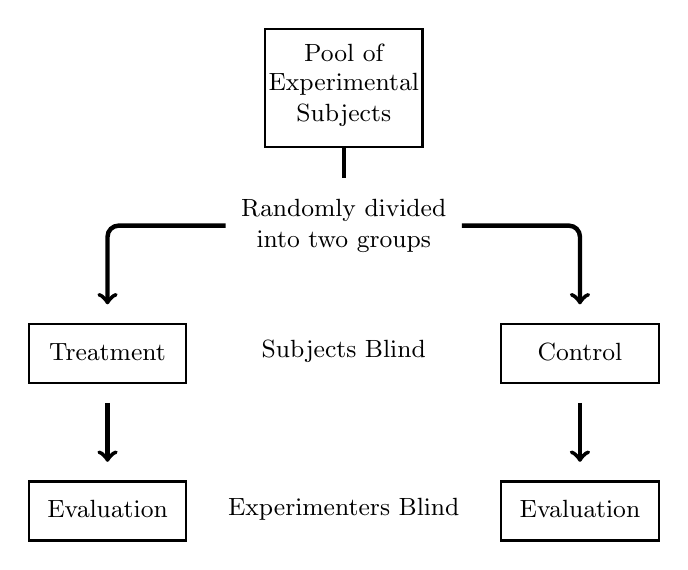
\begin{tikzpicture}
	\draw [thick] (0,0) rectangle (2,1.5);
	\draw [ultra thick] (1,0) -- (1,-0.4);
	\draw [ultra thick, ->, rounded corners] (2.5,-1) -- (4,-1) -- (4, -2);
	\draw [ultra thick, ->, rounded corners] (-0.5,-1) -- (-2,-1) -- (-2, -2);
	\draw [ultra thick, ->] (-2, -3.25) -- (-2, -4); 
	\draw [ultra thick, ->] (4, -3.25) -- (4, -4); 
	\draw [thick] (3,-2.25) rectangle (5,-3);
	\draw [thick] (3,-4.25) rectangle (5,-5);
	\draw [thick] (-3,-2.25) rectangle (-1,-3);
	\draw [thick] (-3,-4.25) rectangle (-1,-5);
	\node [font=\small] at (1,1.2) {Pool of};
	\node [font=\small] at (1,0.8) {Experimental};
	\node [font=\small] at (1,0.4) {Subjects};
	\node [font=\small] at (1,-0.8) {Randomly divided};
	\node [font=\small] at (1,-1.2) {into two groups};
	\node [font=\small] at (1,-2.6) {Subjects Blind};
	\node [font=\small] at (1,-4.6) {Experimenters Blind};
	\node [font=\small] at (4,-2.6) {Control};
	\node [font=\small] at (4,-4.6) {Evaluation};
	\node [font=\small] at (-2,-2.6) {Treatment};
	\node [font=\small] at (-2,-4.6) {Evaluation};
\end{tikzpicture}
\end{figure}
\end{frame}
%%%%%%%%%%%%%%%%%%%%%%%%%%%%%%%%%%%%%%%%
\begin{frame}
\frametitle{Gold Standard: Randomized, Double-blind Experiment}
	\begin{quote}
		Randomized blind experiments ensure that on average the two groups are initially equal, and continue to be treated equally. Thus a fair comparison is possible.
	\end{quote}
	
	\vspace{2em}
	\begin{alertblock}{Randomized, double-blind experiments are generally the best way to untangle causation.}
	\end{alertblock}

	\begin{block}{Sugar Doesn't Make Kids Hyper}
		\href{http://www.youtube.com/watch?v=mkr9YsmrPAI}{http://www.youtube.com/watch?v=mkr9YsmrPAI}
	\end{block}
\end{frame}
%%%%%%%%%%%%%%%%%%%%%%%%%%%%%%%%%%%%%%%%


\begin{frame}
\frametitle{
\includegraphics[scale = 0.05]{./images/clicker} \hfill Racial Bias in Sentencing}
Could we use a randomized experiment to learn whether there is racial discrimination in criminal sentencing?

	\begin{enumerate}[(a)]
		\item Yes
		\item No
	\end{enumerate}
%Please respond using your remote.
\end{frame}
%%%%%%%%%%%%%%%%%%%%%%%%%%%%%%%%%%%%%%%%
\begin{frame}
\frametitle{Randomization is not always possible, practical, or ethical.}


\end{frame}




%%%%%%%%%%%%%%%%%%%%%%%%%%%%%%%%%%%%%%%%

\begin{frame}

\begin{block}{Observational Data}
Data that do not come from a randomized experiment.

\end{block}
\vspace{2em}
\begin{alertblock}{It is very difficult to untangle cause and effect using observational data because of confounders.}
\end{alertblock}


\end{frame}


%%%%%%%%%%%%%%%%%%%%%%%%%%%%%%%%%%%%%%%%

\begin{frame}

\frametitle{Does Racial Discrimination  Affect Criminal Sentencing?}
\framesubtitle{Source: \href{https://www.law.upenn.edu/live/news/2170-new-study-by-professor-david-s-abrams-confirms}{\fbox{Penn Law Website}}}
\footnotesize
\begin{quote}
Social scientists have studied the issue for decades, but the seemingly simple question “Does race affect sentencing?” is surprisingly difficult to answer on the basis of empirical evidence.

Abrams explains: \alert{``The most straightforward way you might look at it is to say, Let’s look at what sentences people get and see whether sentence length varies by race. If it looks like people of one race receive longer sentences than another, that might indicate that the criminal justice system is unfair. But the shortcoming to that approach is that it’s also possible that sentences can differ for many reasons; for example, it’s possible people of different races might have different criminal histories on average, and that could also explain the difference in sentence length''}
\end{quote}
\end{frame}
%%%%%%%%%%%%%%%%%%%%%%%%%%%%%%%%%%%%%%%%
\begin{frame}
\frametitle{Reducing Bias in Observational Studies}
\begin{block}{Regression}
Technique that allows us to remove influence of confounders. Works well if we can identify and gather data on all of them. But...
\end{block}

\end{frame}
%%%%%%%%%%%%%%%%%%%%%%%%%%%%%%%%%%%%%%%%
\begin{frame}
\frametitle{Does Racial Discrimination  Affect Criminal Sentencing?}
\framesubtitle{Source: \href{https://www.law.upenn.edu/live/news/2170-new-study-by-professor-david-s-abrams-confirms}{\fbox{Penn Law Website}}}
\footnotesize
\begin{quote}
To address that difficulty [confounders] social scientists have ... applied control variables to standard regression equations, a statistical method for identifying significant correlations between observed events. For instance, controlling for type of crime committed or for the defendant’s criminal history, researchers look to see whether the results of their equation still show racial disparity.\alert{``The problem with that is you still leave the possibility that any differences you see are due to unobserved variables, differences that might be there but that you can't control for''} Abrams says.``That might be demeanor in the courtroom, it might be the quality of the attorney you can afford, it might be some details about the crime that you might not capture in your data. If those things are correlated with race, which they probably are, you’re not going to know whether the effect you think you’re detecting is really race or is something else''
\end{quote}


\end{frame}


%%%%%%%%%%%%%%%%%%%%%%%%%%%%%%%%%%%%%%%%

\end{document}
